%
% PARA COMPILARLO Y CREAR EL PDF
%    pdflatex paper.tex && pdflatex paper.tex && pdflatex paper.tex 
%

\documentclass{llncs}
\usepackage{graphics}
\usepackage[dvips]{epsfig}
\usepackage[spanish]{babel}
\usepackage[utf8x]{inputenc} %tildes
\usepackage[T1]{fontenc}
\usepackage[hidelinks]{hyperref}
%\usepackage[latin1]{inputenc} % tildes

\def\CC{{C\hspace{-.05em}\raisebox{.4ex}{\tiny\bf ++}}~}
\addtolength{\textfloatsep}{-0.5cm}
\addtolength{\intextsep}{-0.5cm}


%%%%%%%%%%%%%%%% Título %%%%%%%%%%%%%%%
\title{Open Access: revisión histórica y situación actual}

\author{ Cristina Heredia\inst{*} \and Alejandro Alcalde\inst{*} \and David Charte\thanks{Contribución equitativa} }

\institute{
           Departamento de Ciencias de la Computación e Inteligencia Artificial \\
           Universidad de Granada \\
           Granada, España. \\
           {\tt \{CRIS,ALEX,fdavidcl\}@correo.ugr.es}
}

\date{} 

\begin{document}

\maketitle

\section*{Resumen}
Con el volumen creciente de conocimiento publicado y la creciente proliferación de revistas científicas, muchas editoriales y revistas han optado por hacer negocio de ello pidiendo una retribución a los autores que quieran publicar en sus revistas, pero también a todo usuario que desee leer o acceder esas publicaciones, llegando a veces a solicitar una suscripción. Las revistas y editoriales no escatiman fijando sus precios, por lo que muchas de estas publicaciones son innacesibles por usuarios, escuelas, negocios o incluso algunas instituciones que cuentan con menos capital, por ejemplo, las universidades en India o en cualquier país en vía de desarrollo.     

En este artículo se habla del open acces como solución a esas fronteras que limitan el acceso a la información. Se hablará del modelo tradicional de publicación y las amenazas que este presenta actualmente, trataremos distintas soluciones e iniciativas y hablaremos de la legislación a favor de este modo de acceso a la información.
 
\section{Introducción}

Fue en 1665 cuando aparecieron las primeras revistas científicas en París y Londres y ya entonces a los autores no se les retribuía por publicar en ellas. El éxito de estas revistas tras su aparición fue directo, pues los lectores encontaron una forma de leer el trabajo de otras personas más rápido que leyendo un libro,  
mientras que los autores vieron en ellas una buena oportunidad de compartir sus últimos trabajos con todo el mundo de forma rápida, y así poder ser priorizados entre otros científicos, por lo que comenzaron a escribir por impacto y no por dinero. Durante los años posteriores a su aparición, los precios de las revistas impresas crecieron hasta volverse inasequibles para la gran mayoría, y fortuitamente apareció internet para ofrecer una alternativa a tan elevados precios. Esta crisis de precios, junto con el aumento del número de publicaciones científicas, fue un factor importante en la aparición del \textbf{open access}.
\newline
\newline
\textbf{Open access} es una forma de acceder a la información, por tanto no es un modelo de negocio, ni un tipo de licencia ni de contenido. En literatura de investigación, el open access se compone de copias online disponibles para todo el mundo y de forma gratuita de artículos, conferencias, informes técnicos, tesis y documentos de trabajo. Aunque en la mayoría de los casos no tienen restricciones de uso por parte de los usuarios, pudiendo usarse para investigar sobre ellos, docencia u otros propósitos, el open acces no es incompatible con el uso de copyright.\newline 
Por tanto, el open access trata de ofrecer una alternativa mejor al modelo tradicional de publicación, en el que los autores pagan por publicar sus investigaciones y los lectores deben pagar, dependendiendo de la editorial, un precio significativo para poder accederlas, con el fin de romper esa barrera y hacer esa información accesible a personas o instituciones que no puedan afrontar pagar por ese conocimiento.
\newline
Según \cite{suber2007open} las tres principales maneras de proveer open access por los investigadores, son: dejar una copia del artículo en un archivo o repositorio open access (por ejemplo arXiv), publicar en revistas open access (por ejemplo BioMed o las de Public Library of Science) o poner una copia del artículo en una web personal o de departamento. Otra forma de open access son las revistas "híbridas", donde el autor además de pagar por publicar, puede pagar por hacer su artículo accesible a todo el mundo online. Normalmente, las revistas open access usan un código de color para calificar las revistas, donde \textit{dorado} significa que provee open access sin retraso, \textit{verde} indica que permite el archivo de trabajos ya publicados, \textit{verde pálido} indica que permite el archivo de trabajos que se han mandado a revisión pero que aún no se hayan publicado, y \textit{gris} que indica que no cumple ninguna de las anteriores.

 


La sección~\ref{amenazas} describe algunas amenazas que presenta el sistema actual, centrándose en Elsevier, que es una de las editoriales más problemática en este aspecto \cite{costknowledge}. A continuación, la sección~\ref{iniciativas} recoge iniciativas a favor del acceso abierto a la ciencia.

\section{Modelo tradicional: problemática y escándalos}\label{amenazas}

Antes de la era de la información y tecnología, el rol de las revistas científicas era múltiple. El principal era la divulgación de las investigaciones científicas. Las revistas cobraban el coste de la maquetación, el cual no era sencillo para matemáticas, el coste de publicar en formato físico y el de distribución de los mismos a los suscriptores. En la era digital, nada de esto supone un coste tan elevado. De hecho, ahora son los propios investigadores quienes maquetan el documento de forma electrónica, el coste de publicar y distribuir no es para nada comparable con los del pasado. Y lo más importante, la divulgación de las investigaciones ya no se hace de forma física, sino electrónica. Esto no quiere decir que la divulgación sea gratuita, si no que es mucho más barata.

En resumen, el coste de publicación para una revista se ha desplomado debido a que la maquetación han pasado a hacerla los autores y la publicación y distribución ha decrementado significativamente. Por contra, la cantidad de dinero que gastan las bibliotecas universitarias en revistas se ha incrementado. La pregunta entonces es, ¿Por qué siguen los científicos haciendo la labor de revisores y editores de forma volutaria, mientras las universidades pagan todo ese dinero por un servicio que no justifica ese coste?

Esto se debe principalmente a cómo funciona el mundo académico. En resumen, si un investigador quiere avanzar en su carrera, debe tener publicaciones de calidad en revistas de calidad. Por esta razón es difícil cambiar a otro modelo. Una razón es que no es posible crear una nueva revista y esperar a que los investigadores publiquen en ella, ya que si no tiene reputación, no van a considerarla.

Tanto Elsevier, Springer como otras muchas editoriales explotan la labor voluntaria de los investigadores para obtener un beneficio económico muy elevado. Aunque proporcionan un servicio, el precio no está para nada justificado.

Aunque Elsevier quizá no sea la más cara de todas, ha estado implicada en muchos escándalos que la ponen en el punto de mira. Es por ello que muchos investigadores han iniciado un boicot contra ella, como se menciona en la sección~\ref{sec:boicot}

Comencemos con el problema del coste de la revista. Es difícil realizar comparaciones en este aspecto, ya que las distintas revistas varían en el número de páginas por volumen e incluso la cantidad de texto por páginas. Una aproximación tomada por \cite{costknowledge} es calcular el precio por página. Con esta métrica, la revista más rentable a la par que reputada es \textit{The Annals of Mathematics} con \$0.13/página. Elsevier sin embargo tiene un coste de \$1.30/página.

Además de ser una de las más caras, Elsevier ha estado involucrada en una serie de escándalos que no la dejan en buen lugar con respecto a su contenido científico. Un ejemplo involucra a la revista \textit{Chaos, Solitions \& Fractals}, una de las revistas con mayor factor de impacto hasta que se descubrió el escándalo. Este gran factor de impacto se debía a que la revista publicaba muchos papers llenos de citaciones mutuas, además de ser el contenido de dichos papers poco rigurosos.

Elsevier se vio implicado en otro escándalo, esta vez en el campo de la medicina, en el que recibió dinero de la industria farmacéutica para publicar una serie de artículos patrocinados.

Los ejemplos anteriores son solo una demostración de los tipos de escándalos en los que Elsevier ha estado involucrada, hay bastantes más. Esto demuestra que Elsevier solo quiere ganar dinero, y no está interesada realmente en el avance científico.

\section{Open Access: soluciones e iniciativas}\label{iniciativas}

Desde la publicación del manifiesto de la Budapest OA Initiative \cite{boai} en 2002, han surgido distintas iniciativas que tratan de promover la publicación científica en acceso abierto. Estos estímulos proceden de distintas fuentes, tanto del ámbito gubernamental como el editorial, e incluso de personas concretas cuyos proyectos han afectado al curso del acceso libre a la ciencia.

\subsection{Iniciativas en el ámbito de la investigación}

Diferentes editoriales han puesto en marcha la creación de revistas de acceso abierto (\textit{Open Access Journals, OAJ}). El primer OAJ fue \textit{New Horizons in Adult Education} de la editorial Wiley \cite{earlyoaj}, fundado en 1987. Le siguieron \textit{Psycoloquy} y \textit{Public Access-Computer Systems Review} en 1989. A partir de 1990, fueron surgiendo más OAJs de forma incremental. En la actualidad, el \textit{Directory of Open Access Journals}\footnote{Disponible en \url{https://doaj.org/}, accedido el 29 de noviembre de 2017.}, creado y mantenido originalmente por la universidad de Lund \cite{nordic}, contabiliza un total de 10544 revistas de acceso abierto. En la fig.~\ref{fig:doaj} se muestra el total de OAJs que se han puesto a disposición pública en el directorio a lo largo del tiempo. Se puede observar que el crecimiento se acentúa progresivamente conforme avanzan los años.

\begin{figure}[htbp]
  \centering
  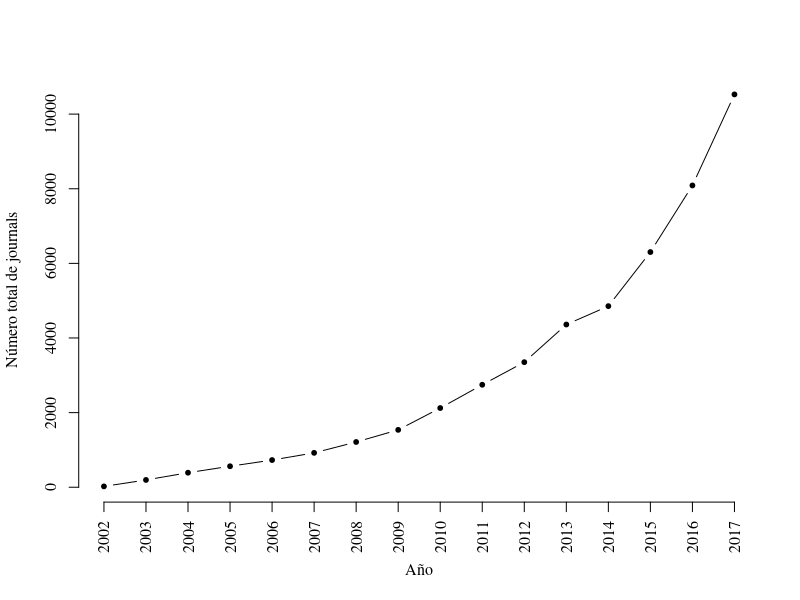
\includegraphics[width=0.8\textwidth]{doaj_years.png}
  \caption{\label{fig:doaj}Total de OAJs listados en el \textit{Directory of Open Access Journals} desde su creación en 2002. Datos de \url{https://doaj.org/csv}}

\end{figure}

\label{sec:boicot}
Otra de las iniciativas que han marcado un impacto en el progreso del acceso abierto ha sido el boicot a editoriales y lobbies anti-Open Access, como Elsevier \cite{costknowledge}. En particular, una de las acciones más impactantes fue la renuncia del equipo editorial al completo del conocido journal \textit{Lingua} de Elsevier sobre lingüística, para después fundar un nuevo OAJ orientado a la misma temática, \textit{Glossa} \cite{linguaglossa}.

%- BioMed Central
%- Nucleic Acids Research (OUP)
%- Molecular Systems Biology (Nature)

\subsection{Legislación a favor del Open Access}


Estados Unidos aprobó en 2013 el \textit{Fair Access to Science and Technology Research Act} \cite{fastr}, que implica que las agencias gubernamentales que destinen más de 100 millones de dólares anuales a investigación deben publicar los resultados para acceso abierto en un plazo razonable. % Asimismo, el National Institutes of Health publica toda la investigación obtenida en PubMed Central en menos de 12 meses.

Reino Unido tiene vigente desde 2012 una legislación que fuerza a que todo el trabajo financiado por el Department for International Development sea publicado de forma abierta en un plazo de 2 años desde su publicación en revista \cite{ukdifd}. Además, los Research Councils proporcionan financiación a las instituciones académicas para sufragar los costes de publicación en Open Access tipo Gold\cite{rcuk}.

En la Unión Europea han puesto en marcha acuerdos que llevarían a una legislación que permitiría tener todas las publicaciones científicas financiadas de forma pública accesibles libremente para el año 2020 \cite{enserink2016dramatic}. Este proyecto surge de una llamada a la acción por parte del gobierno neerlandés \cite{amsterdam}.

\subsection{Iniciativas independientes}

Algunas de las acciones más notorias a favor del Open Access han sido propiciadas por activistas individuales. Aaron Swartz fue un activista que escribió el Guerilla Open Access Manifesto \cite{goam} a favor del libre intercambio de todo tipo de conocimiento, y en particular del obtenido a partir de la investigación científica. Alrededor de este manifiesto ha surgido un movimiento homónimo \cite{pirates}, con diferentes iniciativas y ataques a los obstáculos al libre acceso a la investigación.

El servicio web Sci-Hub\footnote{Disponible en \url{https://sci-hub.bz} en el momento en que se escribió este trabajo, previamente accesible en \url{https://sci-hub.cc} y \url{https://sci-hub.io}}, desarrollado en 2011 por Alexandra Elbakyan, es un buscador de publicaciones científicas que accede a los portales de descarga de las mismas mediante credenciales filtradas de distintas instituciones \cite{himmelstein-scihub}, de forma que el usuario puede descargarlas sin estar identificado en una institución suscrita a la revista correspondiente. El impacto de Sci-Hub ha sido notable, tanto que algunos analistas presagian el fin de las publicaciones académicas bajo suscripción \cite{sciencescihub}.

%% \begin{quote}
%%  We need to take information, wherever it is stored, make our copies and share them with
%% the world. We need to take stuff that's out of copyright and add it to the archive. We need
%% to buy secret databases and put them on the Web. We need to download scientific
%% journals and upload them to file sharing networks.

%% --- Aaron Swartz, Guerilla Open Access Manifesto \cite{goam}
%% \end{quote}

\section{Comentarios finales}

En este trabajo se ha estudiado el modelo tradicional de publicaciones científicas y los avances que ha habido a lo largo del tiempo para transformarlo en un modelo de acceso abierto. Se ha observado cómo el comportamiento de las editoriales que se aferran a las \textit{paywalls} no es siempre el más propicio para una ciencia rigurosa. Finalmente, se han analizado ataques al modelo tradicional e iniciativas en distintos campos, que podrían llevar a la ciencia a un futuro donde la investigación sea accesible para todas las personas.

%%%%%%%%%%%%%% Bibliografy %%%%%%%%%%%%%%%
\bibliographystyle{splncs}
\bibliography{refs}

\end{document}
